\section{Smart Contracts}
\label{sec:smart-contract}

Smart Contracts adalah sebuah protokol transaksi elektronik yang mengeksekusi kesepakatan dari sebuah kontrak. Klausa kesepakatan yang dimasukkan ke dalam sebuah Smart Contract akan diberlakukan secara otomatis saat kondisi yang sesuai sudah tercapai. Sehingga, suatu pihak yang melanggar kontrak akan dihukum secara otomatis. Smart Contract adalah sebuah cara untuk meminimalisir kepercayaan kepada perantara pihak ketiga sebagai \textit{enforcer} dari sebuah kontrak \parencite{szabo1997formalizing}.

Smart Contracts adalah salah satu teknologi yang dimungkinkan oleh teknologi Blockchain. Seluruh klausa kontraktual dalam sebuah Smart Contract akan dikonversi menjadi sebuah bentuk \textit{executable computer programs}. Seluruh eksekusi dari setiap \textit{contract statement} direkam dan dimasukkan ke dalam transaksi yang \textit{immutable}, yang disimpan di dalam Blockchain. Smart Contracts juga dapat menjamin \textit{access control} yang tepat dan \textit{contract enforcement} yang deterministik, karena dijamin dalam seluruh \textit{logic} yang terdapat di dalam Smart Contract tersebut \parencite{zheng2020overview}.

\begin{figure}[ht]
	\centering
	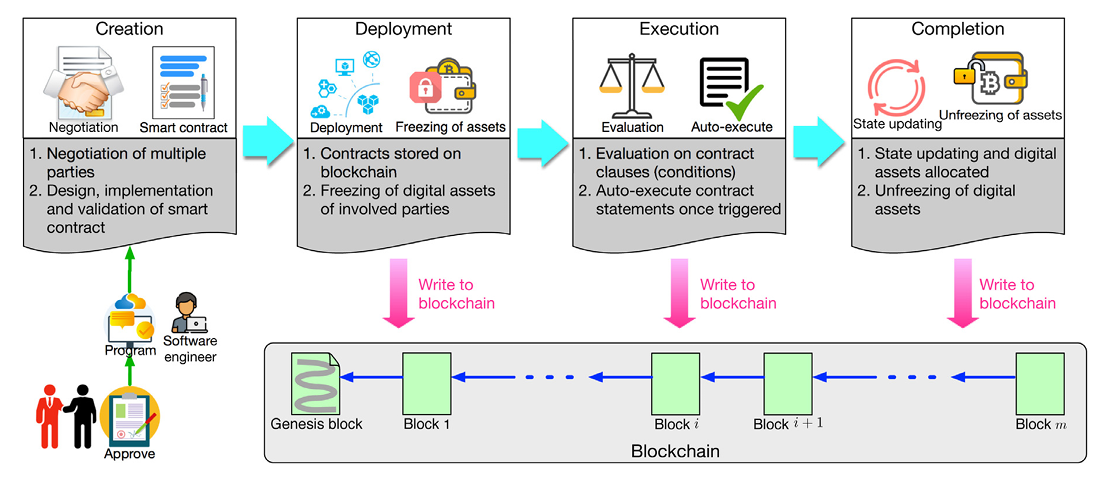
\includegraphics[width=0.7\textwidth]{resources/chapter-2/sc-lifecycle.png}
	\caption{\textit{Life cycle} dari Smart Contract \parencite{zheng2020overview}}
	\label{image:sc-lifecycle}
\end{figure}

\textit{Life cycle} dari sebuah Smart Contract terdiri dari empat fase seperti pada ilustrasi di Gambar \ref{image:sc-lifecycle}:

\begin{enumerate}
	\item \textit{Creation}: negosiasi antar pihak untuk menyepakati ketentuan dari kontrak dalam \textit{natural language}, dan translasi menjadi Smart Contracts.
	\item \textit{Deployment}: kontrak yang sudah divalidasi dapat disimpan ke dalam Blockchain, menjadikannya tidak bisa dimodifikasi.
	\item \textit{Execution}: Setelah \textit{deployment}, klausa kontraktual akan dimonitor, dan saat kondisi yang sesuai dengan yang terdefinisi dalam Smart Contract, maka prosedur kontrak akan dieksekusi secara otomatis.
	\item \textit{Completion}: Setelah eksekusi, \textit{state} baru dari semua pihak akan diperbarui sesuai dengan hasil dari transaksi yang terjadi dan disimpan ke dalam Blockchain. 
\end{enumerate}

\subsection{Off-Chain Smart Contracts}
\label{subsec:off-chain-smart-contracts}

\textit{Off-chain Smart Contract} adalah Smart Contracts yang dieksekusi diluar Blockchain, \textit{signed} hanya oleh \textit{interested participants}, dan digunakan untuk mengenkapsulasi fungsi yang melibatkan komputasi \textit{high-cost} atau \textit{private information} terkait \textit{participants}. Terdapat banyak cara untuk tetap menjaga properti dan keuntungan penggunaan dari Blockchain, contohnya, hasil dari eksekusi sebuah \textit{off-chain Smart Contract} dapat dilakukan \textit{logging} pada Blockchain, sehingga jika terjadi \textit{dispute} dalam eksekusi \textit{off-chain Smart Contract}, sebuah \textit{on-chain Smart Contract} dapat digunakan untuk \textit{fork off-chain Smart Contract} dan mengeksekusinya di dalam Blockchain untuk menyelesaikan \textit{dispute} \parencite{zou2019smart}.

\subsection{Semantic Smart Contracts}
\label{subsec:semantic-smart-contracts}
Semantic Smart Contracts adalah sebuah cara untuk merepresentasikan \textit{semantics} dari Smart Contract menggunakan konsep \textit{EthOn contract extension} dan sebuah \textit{vocabulary} yang terkait dengan bisnis. Semantic Smart Contracts mengizinkan untuk membandingkan \textit{request} dengan beberapa \textit{request description} dengan mengonsiderasi semantik dari anotasi yang mereferensikan sebuah \textit{shared domain ontology} \parencite{baqa2019semantic}.
